% =============================================================================
% Poster A0 portret — Disertație Sistem E-Medicine (tikzposter)
% Variantă aerisită + benzi de statistici/stack, fundal tentat.
% Figurile sunt reutilizate vectorial din teză (poster_frags/*.tex)
% Compilare: pdflatex Disertatie_poster.tex
% =============================================================================
\documentclass[25pt, a0paper, portrait, margin=20mm, innermargin=18mm,
               blockverticalspace=20mm, colspace=24mm, subcolspace=10mm]{tikzposter}

\usepackage[T1]{fontenc}
\usepackage{lmodern}
\usepackage[romanian]{babel}
\usepackage{amsmath, amssymb, bm}
\usepackage{booktabs}
\usepackage{tikz}
\usepackage{pgfplots}
\pgfplotsset{compat=1.18}
\usepgfplotslibrary{groupplots}
\usetikzlibrary{arrows.meta, positioning, shapes.geometric, fit, calc}

\newcommand{\Rzero}{\mathcal{R}_0}
\definecolor{petrol}{RGB}{18,74,99}
\definecolor{petroldeschis}{RGB}{30,136,168}
\setlength{\parskip}{9pt}
\renewcommand{\baselinestretch}{1.1}

% ---- stil culori petrol; fundal usor tentat ----
\definecolorstyle{Teza}{}{
  \colorlet{backgroundcolor}{petrol!7}
  \colorlet{framecolor}{petrol}
  \colorlet{titlefgcolor}{white}
  \colorlet{titlebgcolor}{petrol}
  \colorlet{blocktitlebgcolor}{petrol}
  \colorlet{blocktitlefgcolor}{white}
  \colorlet{blockbodybgcolor}{white}
  \colorlet{blockbodyfgcolor}{black}
  \colorlet{innerblocktitlebgcolor}{petroldeschis}
  \colorlet{innerblocktitlefgcolor}{white}
  \colorlet{notebgcolor}{petroldeschis}
  \colorlet{notefgcolor}{white}
}
\usetheme{Default}
\usecolorstyle{Teza}
\usebackgroundstyle{Empty}

% blocuri aerisite: padding interior generos + bara accent stanga
\defineblockstyle{Aer}{
  titlewidthscale=1, bodywidthscale=1, titleleft,
  roundedcorners=16, linewidth=0pt, titleinnersep=14mm, bodyinnersep=16mm
}{
  \draw[draw=none, fill=blockbodybgcolor, rounded corners=\blockroundedcorners]
    (blockbody.south west) rectangle (blockbody.north east);
  \ifBlockHasTitle
    \draw[draw=none, fill=blocktitlebgcolor, rounded corners=\blockroundedcorners]
      (blocktitle.south west) rectangle (blocktitle.north east);
    \draw[line width=11pt, color=petroldeschis]
      ([xshift=5.5pt]blockbody.south west) -- ([xshift=5.5pt]blockbody.north west);
  \fi
}
\useblockstyle{Aer}

% titlu cu 2 randuri explicite (fiecare incape) — tikzposter taie titlul lung
% pe un singur rand, asa ca fortam break-ul manual.
\settitle{
  \centering \vspace*{6mm}
  {\color{titlefgcolor}\bfseries\LARGE
   Sisteme e-medicine de gestionare și monitorizare\\[5mm]
   a datelor epidemiologice\par}
  \vspace{13mm}
  {\color{titlefgcolor}\Large Absolvent: Geană Tudor-Bogdan \quad$\cdot$\quad
   Coordonator științific: Prof. Radu Rădescu\par}
  \vspace{7mm}
  {\color{titlefgcolor}\large Universitatea Națională de Știință și Tehnologie
   POLITEHNICA București \;$\cdot$\; Facultatea de Electronică, Telecomunicații
   și Tehnologia Informației \;$\cdot$\; Lucrare de disertație, Iunie 2026\par}
  \vspace{4mm}
}
\title{Sisteme e-medicine de gestionare și monitorizare a datelor epidemiologice}\author{Geană Tudor-Bogdan}\institute{UNSTPB}

% card de statistica pentru banda de sus
\newcommand{\statcard}[3]{%
  \tikz{\node[rectangle, rounded corners=16pt, fill=#1, draw=petrol, line width=2.5pt,
        minimum width=17.5cm, minimum height=10.5cm, align=center, inner sep=8mm]{%
    \begin{tabular}{c}
      {\fontsize{120}{120}\selectfont\bfseries\color{petrol}#2} \\[6mm]
      {\LARGE\color{black!85} #3}
    \end{tabular}};}}

\begin{document}
\maketitle[roundedcorners=18, linewidth=0pt]

% ===================== BANDA DE STATISTICI (full width) =====================
\begin{columns}
\column{1}
\block{}{%
  \centering
  \resizebox{\linewidth}{!}{%
    \statcard{petrol!12}{8}{compartimente SIDARTHE}\;
    \statcard{petroldeschis!18}{3}{limbaje: R / Julia / Python}\;
    \statcard{petrol!12}{184}{rulări benchmark, 0 eșecuri}\;
    \statcard{petroldeschis!18}{K8s}{cluster real, RF = 3}%
  }
}
\end{columns}

% ===================== CONTINUT PRINCIPAL (3 coloane) =====================
\begin{columns}

% -------- COLOANA 1 --------
\column{0.33}

\block{Context și motivație}{
\Large
Bolile infecțioase sunt un proces \textbf{populațional}. Modelele
compartimentale oferă rigoare matematică, dar costul implementării depinde de
\textbf{limbaj} (R / Julia / Python).

\medskip
\textbf{Scop:} un sistem care leagă \emph{modelarea} de \emph{implementarea
software}, reproductibil și colaborativ.
}

\block{Obiective}{
\Large
\begin{itemize}\setlength{\itemsep}{12pt}
  \item \textbf{SIDARTHE} principal; SIR / SIS / SEIR / SIRS ca repere.
  \item Același contract de simulare în \textbf{R, Julia, Python}.
  \item Metodologie de \textbf{comparație și calibrare}.
  \item Extensie predictivă \textbf{LSTM}.
\end{itemize}
}

\block{Modele compartimentale}{
\centering
\resizebox{\linewidth}{!}{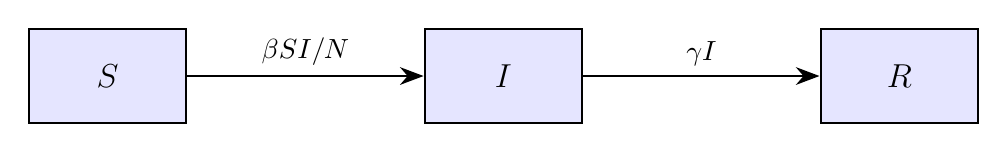
\begin{tikzpicture}[
    box/.style = {rectangle, draw, thick, minimum width=2cm, minimum height=1.2cm,
                  fill=blue!10, font=\large\bfseries},
    arr/.style = {-{Stealth[length=3mm]}, thick},
    lbl/.style = {font=\normalsize, midway, above}
]
    \node[box] (S) {$S$};
    \node[box, right=3cm of S] (I) {$I$};
    \node[box, right=3cm of I] (R) {$R$};

    \draw[arr] (S) -- (I) node[lbl] {$\beta SI/N$};
    \draw[arr] (I) -- (R) node[lbl] {$\gamma I$};
\end{tikzpicture}
}
\par\vspace{12mm}
{\Large $\Rzero = \beta/\gamma$ \;\; (epidemie dacă $\Rzero > 1$)}
\par\vspace{10mm}\Large\raggedright
\textbf{SIDARTHE:} 8 compartimente, 16 rate --- separă diagnosticul,
severitatea clinică și decesele.
}

% -------- COLOANA 2 --------
\column{0.34}

\block{Arhitectura sistemului}{
\centering
\resizebox{!}{20cm}{% Diagrama de arhitectura redesenata pentru poster (curata, fara incrucisari)
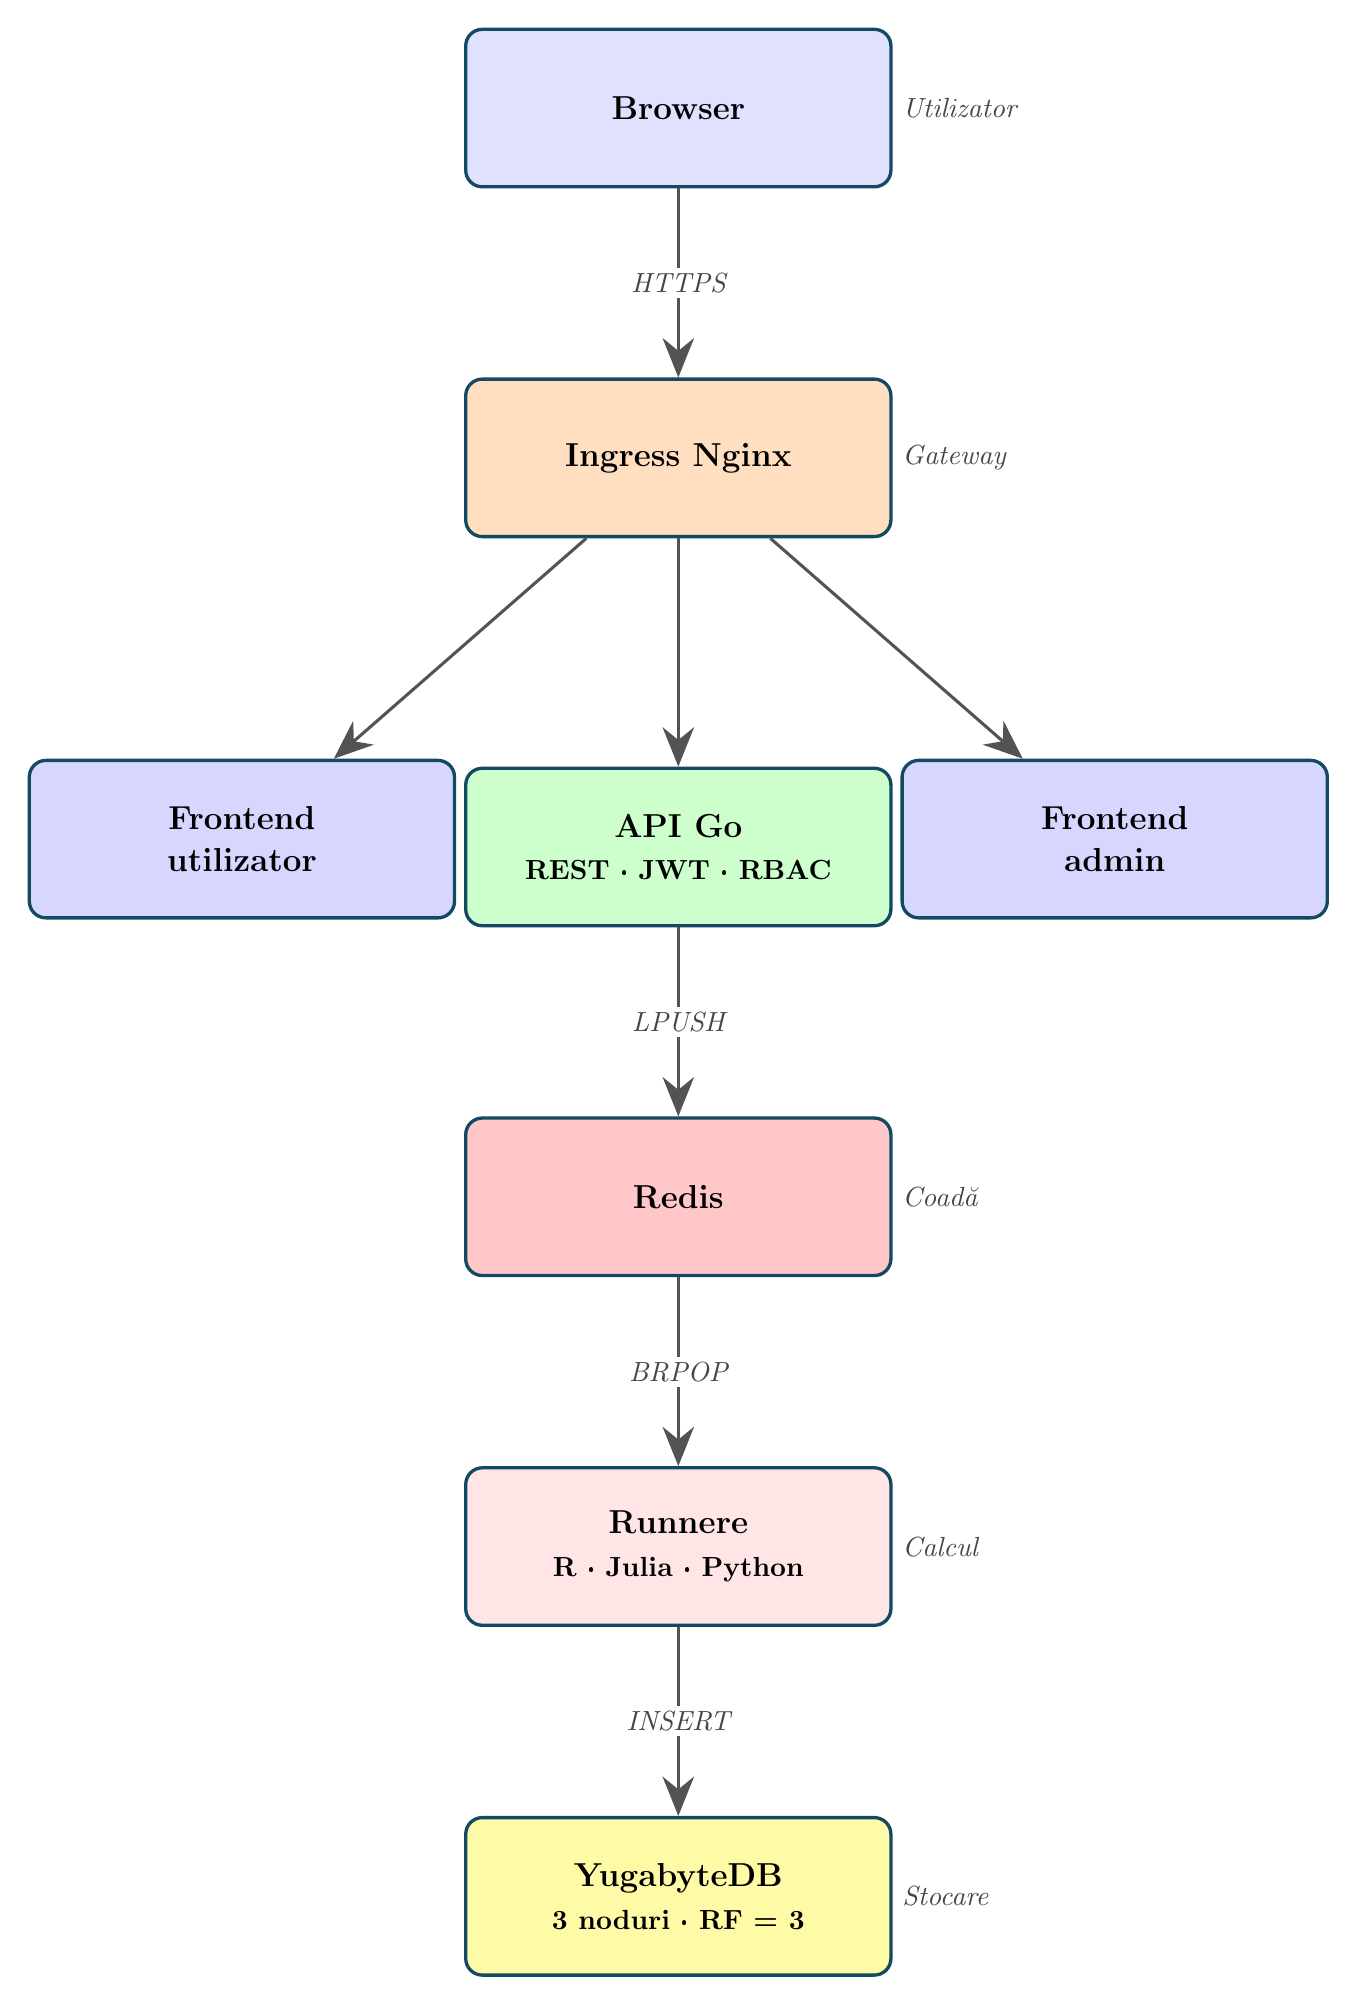
\begin{tikzpicture}[
  box/.style 2 args={rectangle, rounded corners=6pt, draw=petrol, line width=1.2pt,
        minimum width=5.4cm, minimum height=2.0cm, align=center, fill=#1,
        font=\large\bfseries, text=black, label={[font=\normalsize\itshape,
        text=gray!55!black]right:#2}},
  plain/.style={rectangle, rounded corners=6pt, draw=petrol, line width=1.2pt,
        minimum width=5.4cm, minimum height=2.0cm, align=center, fill=#1,
        font=\large\bfseries},
  lbl/.style={font=\normalsize\itshape, text=gray!55!black, midway,
        fill=white, inner sep=2pt},
  ar/.style={-{Stealth[length=5mm,width=4mm]}, line width=1.1pt, gray!65!black},
  node distance=2.4cm and 1.4cm
]
  \node[box={blue!12}{Utilizator}] (browser) {Browser};
  \node[box={orange!25}{Gateway}, below=of browser] (ingress) {Ingress Nginx};

  \node[plain={blue!16}, below left=2.8cm and 0.1cm of ingress] (fu)
        {Frontend\\utilizator};
  \node[box={green!20}{Aplica\c tie}, below=2.9cm of ingress] (api)
        {API Go\\{\normalsize REST · JWT · RBAC}};
  \node[plain={blue!16}, below right=2.8cm and 0.1cm of ingress] (fa)
        {Frontend\\admin};

  \node[box={red!22}{Coad\u a}, below=of api] (redis) {Redis};
  \node[box={red!10}{Calcul}, below=of redis] (run)
        {Runnere\\{\normalsize R · Julia · Python}};
  \node[box={yellow!35}{Stocare}, below=of run] (db)
        {YugabyteDB\\{\normalsize 3 noduri · RF = 3}};

  \draw[ar] (browser) -- (ingress) node[lbl]{HTTPS};
  \draw[ar] (ingress) -- (fu);
  \draw[ar] (ingress) -- (api);
  \draw[ar] (ingress) -- (fa);
  \draw[ar] (api) -- (redis) node[lbl]{LPUSH};
  \draw[ar] (redis) -- (run) node[lbl]{BRPOP};
  \draw[ar] (run) -- (db) node[lbl]{INSERT};
\end{tikzpicture}
}
\par\vspace{8mm}\raggedright\Large
Flux complet de simulare, asincron --- două interfețe Vue.js peste același API.
}

\block{Trei limbaje, un contract}{
\Large
\begin{itemize}\setlength{\itemsep}{12pt}
  \item \textbf{R} --- deSolve (RK4)
  \item \textbf{Julia} --- DifferentialEquations.jl (Tsit5)
  \item \textbf{Python} --- SciPy solve\_ivp (RK45)
\end{itemize}
\medskip
Același mesaj Redis, aceeași schemă JSONB --- \textbf{interschimbabile}.
}

% bloc evidentiat (contributie) — fundal accent
{\colorlet{blockbodybgcolor}{petroldeschis}\colorlet{blockbodyfgcolor}{white}
\block{Contribuție: sistem de plug-in-uri}{
\Large
Super-adminul înregistrează un \textbf{script Python} sau o \textbf{imagine
container} $\rightarrow$ Deployment Kubernetes automat. Plus editor de cod
(Monaco) în interfață.

\medskip
\textbf{Orice algoritm} cu un contract minimal de I/O, fără modificări la API.
}}

% -------- COLOANA 3 --------
\column{0.33}

\block{Rezultate: benchmark}{
\Large \textbf{180 rulări ODE + 4 LSTM}, fără eșecuri, pe cluster Kubernetes.
\par\vspace{10mm}
\centering\large
\begin{tabular}{@{}lcl@{}}
\toprule
\textbf{Limbaj} & \textbf{@\,10k} & \textbf{Profil} \\
\midrule
Julia  & 5--6 ms      & rapid; JIT $\sim$1 s \\
Python & 4--9 ms      & stabil \\
R      & 0,7--1,3 s   & inserții DB \\
\bottomrule
\end{tabular}
\par\vspace{8mm}\raggedright\Large
LSTM evaluat onest: persistența domină la 1 zi (85\% zile plate).
}

\block{Calibrare pe date reale}{
\centering
\resizebox{\linewidth}{!}{\begin{tikzpicture}
\begin{groupplot}[
    group style={
        group size=2 by 2,
        horizontal sep=1.7cm,
        vertical sep=2.4cm,
        ylabels at=edge left,
    },
    width=0.45\textwidth,
    height=4.4cm,
    xlabel={Zi (de la $15$ martie 2020)},
    ylabel={Cazuri active},
    xmin=0, xmax=185,
    ymin=0,
    grid=both, grid style={line width=.1pt, draw=gray!20},
    tick label style={font=\scriptsize},
    label style={font=\scriptsize},
    title style={font=\small\bfseries, yshift=0.4ex},
    legend style={font=\tiny, fill=white, draw=gray!50, at={(0.02, 0.98)}, anchor=north west},
    legend cell align={left},
    every axis plot/.append style={line width=0.6pt},
]
% --- România ---
\nextgroupplot[title={România ($N=19{,}7$ mil., $\hat{\mathcal{R}}_0=1{,}45$)}, ymax=22000]
\draw[dashed, gray!70] (axis cs:154, 0) -- (axis cs:154, 22000);
\addplot[black] table[col sep=comma, x=day, y=obs_romania]
    {data/calibration_multiregion.csv}; \addlegendentry{observat}
\addplot[red!80!black] table[col sep=comma, x=day, y=fit_romania]
    {data/calibration_multiregion.csv}; \addlegendentry{fit (train)}
\addplot[red!70!black, dashed] table[col sep=comma, x=day, y=pred_romania]
    {data/calibration_multiregion.csv}; \addlegendentry{prognoza (test)}

% --- Italia ---
\nextgroupplot[title={Italia ($N=59{,}0$ mil., $\hat{\mathcal{R}}_0=0{,}94$)}, ymax=120000]
\draw[dashed, gray!70] (axis cs:154, 0) -- (axis cs:154, 120000);
\addplot[black] table[col sep=comma, x=day, y=obs_italy]
    {data/calibration_multiregion.csv};
\addplot[red!80!black] table[col sep=comma, x=day, y=fit_italy]
    {data/calibration_multiregion.csv};
\addplot[red!70!black, dashed] table[col sep=comma, x=day, y=pred_italy]
    {data/calibration_multiregion.csv};

% --- Germania ---
\nextgroupplot[title={Germania ($N=83{,}4$ mil., $\hat{\mathcal{R}}_0=1{,}05$)}, ymax=30000]
\draw[dashed, gray!70] (axis cs:154, 0) -- (axis cs:154, 30000);
\addplot[black] table[col sep=comma, x=day, y=obs_germany]
    {data/calibration_multiregion.csv};
\addplot[red!80!black] table[col sep=comma, x=day, y=fit_germany]
    {data/calibration_multiregion.csv};
\addplot[red!70!black, dashed] table[col sep=comma, x=day, y=pred_germany]
    {data/calibration_multiregion.csv};

% --- Spania ---
\nextgroupplot[title={Spania ($N=47{,}6$ mil., $\hat{\mathcal{R}}_0=1{,}06$)}, ymax=160000]
\draw[dashed, gray!70] (axis cs:154, 0) -- (axis cs:154, 160000);
\addplot[black] table[col sep=comma, x=day, y=obs_spain]
    {data/calibration_multiregion.csv};
\addplot[red!80!black] table[col sep=comma, x=day, y=fit_spain]
    {data/calibration_multiregion.csv};
\addplot[red!70!black, dashed] table[col sep=comma, x=day, y=pred_spain]
    {data/calibration_multiregion.csv};

\end{groupplot}
\end{tikzpicture}
}
\par\vspace{8mm}\raggedright\Large
SIR pe valul 1 COVID-19, 4 țări: $\Rzero$ între \textbf{0,94} și \textbf{1,45}.
}

\block{Concluzii}{
\Large
\begin{itemize}\setlength{\itemsep}{12pt}
  \item Lanț complet: modelare $\to$ implementare $\to$ arhitectură.
  \item Benchmarking cross-limbaj + calibrare reală + platformă web cu RBAC.
  \item Deployat pe cluster Kubernetes real (YugabyteDB RF\,=\,3).
\end{itemize}
}

\end{columns}

% ===================== BANDA DE JOS: STACK (full width) =====================
\begin{columns}
\column{1}
{\colorlet{blockbodybgcolor}{petrol}\colorlet{blockbodyfgcolor}{white}
\block{}{%
  \centering\LARGE
  \textbf{Stack tehnologic:}\;\; Go (chi · pgx) \,$\cdot$\, Vue 3 + TypeScript
  \,$\cdot$\, YugabyteDB \,$\cdot$\, Redis \,$\cdot$\, Kubernetes \,$\cdot$\,
  R / Julia / Python \,$\cdot$\, LSTM (NumPy)
}}
\end{columns}

\end{document}
